\chapter{Revisão de litaratura}

\label{cap:literatura}

Nossa revisão de literatura aborda predominantemente três temas. O primeiro deles é uma revisão da estrutura geral e estimação dos parâmetros de um modelo multivariado de covariância linear generalizada, baseado nas ideias de \citet{Bonat16}. A segunda parte da revisão de literatura diz respeito ao procedimento dos chamados testes de hipóteses com o foco de tratar do objetivo, notação, componentes, aplicação deste tipo de procedimento no contexto de modelos de regressão e ainda quais os testes mais comuns. Por fim, a última parte da revisão diz respeito às análises de variância, que podem ser vistos como procedimentos baseados em testes de hipóteses sequenciais para avaliar os parâmetros de um modelo de regressão.

\section{Modelos Multivariados de Covariância Linear Generalizada}

Os modelos linerares generalizados (GLM), propostos por \citet{Nelder72}, são uma forma de modelagem que lida exclusivamente com uma resposta e com respostas de diferentes naturezas, tais como respostas contínuas, binárias e contagens. Tais características tornam essa classe de modelos uma flexível ferramenta de modelagem aplicável a diversos tipos de problemas. Contudo, por mais flexível e discutida na literatura, essa classe apresenta ao menos três importantes restrições: um leque restrito de distribuições disponíveis para modelagem, a incapacidade de lidar com observações dependentes e a incapacidade de lidar com múltiplas respostas simultaneamente. 

Com o objetivo de contornar estas restrições, foi proposta por \citet{Bonat16}, uma estrutura geral para análise de dados não gaussianos com múltiplas respostas em que não se faz suposições quanto à independência das observações: os chamados modelos multivariados de covariância linear generalizada (McGLMs). Tais modelos, levam em conta a não normalidade por meio de uma função de variância. Além disso, a estrutura média é modelada por meio de uma função de ligação e um preditor linear. Os parâmetros dos modelos são obtidos através de funções de estimação baseadas em suposições de segundo momento.

Vamos discutir os McGLMs como uma extensão dos GLMs. Vale ressaltar que é usada uma especificação menos usual de um modelo linear generalizado, porém trata-se de uma notação mais conveniente para chegar à uma especificação mais simples de um modelo multivariado de covariância linear generalizada.

\subsection{Modelo linear generalizado}

Para definição da extensão de um modelo linear generalizdo (GLM) apresentada por \citet{Bonat16}, considere $\boldsymbol{Y}$ um vetor $N \times 1$ de valores observados da variável resposta, $\boldsymbol{X}$ uma matriz de delineamento $N \times k$ e $\boldsymbol{\beta}$ um vetor de parâmetros de regressão $k \times 1$. Com isso, um GLM pode ser escrito da seguinte forma 

\begin{equation}
\label{eq:glm}
      \begin{aligned}
        \mathrm{E}(\boldsymbol{Y}) &=
         \boldsymbol{\mu} =
            g^{-1}(\boldsymbol{X} \boldsymbol{\beta}),
            \\
        \mathrm{Var}(\boldsymbol{Y}) &=
          \Sigma =
          \mathrm{V}\left(\boldsymbol{\mu}; p\right)^{1/2}\left(\tau_0\boldsymbol{I}\right)\mathrm{V}\left(\boldsymbol{\mu}; p\right)^{1/2},
      \end{aligned}
\end{equation}

\noindent em que $g(.)$ é a função de ligação, $\mathrm{V}\left(\boldsymbol{\mu}; p\right)$ é uma matriz diagonal em que as entradas principais são dadas pela função de variância aplicada ao vetor $\boldsymbol{\mu}$, $p$ é o parâmetro de potência, $\tau_0$ o parâmetro de dispersão e $\boldsymbol{I}$ é a matriz identidade de ordem $N\times N$.

Nesta extensão, os GLMs fazem uso de apenas duas funções, a função de variância e de ligação. Diferentes escolhas de funções de variância implicam em diferentes suposições a respeito da distribuição da variável resposta. Dentre as funções de variância conhecidas, podemos citar:

1. A função de variância potência, que caracteriza a família Tweedie de distribuições, em que a função de variância é dada por $\vartheta\left(\boldsymbol{\mu}; p\right) = \mu^p$, na qual destacam-se as distribuições: normal ($p$ = 0), Poisson ($p$ = 1), gama ($p$ = 2) e  normal inversa ($p$ = 3). Para mais informações consulte \citet{Jorgensen87} e \citet{Jorgensen97}.

2. A função de dispersão Poisson–Tweedie, a qual caracteriza a família Poisson-Tweedie de distribuições, que visa contornar a inflexibilidade da utilização da função de variância potência para  respostas discretas. A família Poisson-Tweedie tem função de dispersão dada por $\vartheta\left(\boldsymbol{\mu}; p\right) = \mu + \mu^p$ e tem como casos particulares os mais famosos modelos para dados de contagem: Hermite ($p$ = 0), Neyman tipo A ($p$ = 1), binomial negativa ($p$ = 2) e Poisson–inversa gaussiana (p = $3$) \citep{Jorgensen15}. Não se trata de uma função de variância usual, mas é uma função que caracteriza o relacionamento entre média e variância.

3. A função de variância binomial, dada por $\vartheta(\boldsymbol{\mu}) = \mu(1 - \mu)$, utilizada quando a variável resposta é binária, restrita a um intervalo ou quando tem-se o  número de sucessos em um número de tentativas.

Lembre-se que o GLM é uma classe de modelos de regressão univariados em que um dos pressupostos é a independência entre as observações. Esta independência é especificada na matriz identidade no centro \autoref{eq:glm}. Podemos imaginar que, substituindo esta matriz identidade por uma matriz qualquer que reflita a relação entre os indivíduos da amostra teremos uma extensão do Modelo Linear Generalizado para observações dependentes. É justamente essa a ideia dos modelos de covariância linear generalizada, o cGLM.

\subsection{Modelo de covariância linear generalizada}

Os modelos de covariância linear generalizada (cGLM) são uma alternativa para problemas em que a suposição de independência entre as observações não é atendida. Neste caso, a solução proposta é substituir a matriz identidade $\boldsymbol{I}$ da \autoref{eq:glm} por uma matriz não diagonal $\boldsymbol{\Omega({\tau})}$ que descreva adequadamente a estrutura de correlação entre as observações. Trata-se de uma ideia similar à proposta de \citet{Liang86} nos modelos GEE (Equações de Estimação Generalizadas), em que utiliza-se uma matriz de correlação de trabalho para considerar a dependência entre as observações. A matriz $\boldsymbol{\Omega({\tau})}$ é descrita como uma combinação de matrizes conhecidas tal como nas propostas de \citet{Anderson73} e \citet{Pourahmadi00}, podendo ser escrita da forma

\begin{equation}
\label{eq:cov}
h\left \{ \boldsymbol{\Omega}(\boldsymbol{\tau}) \right \} = \tau_0Z_0 + \ldots + \tau_DZ_D,
\end{equation}

\noindent em que $h(.)$ é a função de ligação de covariância, $Z_d$ com $d$ = 0,$\ldots$, D são matrizes que representam a estrutura de covariância presente nos dados e $\boldsymbol{\tau}$ = $(\tau_0, \ldots, \tau_D)$ é um vetor $(D + 1) \times 1$ de parâmetros de dispersão. Tal estrutura pode ser vista como um análogo ao preditor linear para a média e foi nomeado como preditor linear matricial, a especificação da função de ligação de covariância é discutida por \citet{Pinheiro96}. É possível selecionar combinações de matrizes para se obter os mais conhecidos modelos da literatura para dados longitudinais, séries temporais, dados espaciais e espaço-temporais. Maiores detalhes são discutidos por \citet{Demidenko13}.

Com isso, substituindo a matriz identidade da \autoref{eq:glm} pela \autoref{eq:cov}, temos uma classe com toda a flexibilidade dos GLMs, porém contornando a restrição da independência entre as observações desde que o preditor linear matricial seja adequadamente especificado. Deste modo, é contornada a restrição da incapacidade de lidar com observações dependentes. Outra restrição diz respeito às múltiplas respostas e, contornando este problema, chegamos ao McGLM.

\subsection{Modelos multivariados de covariância linear generalizada}

Os modelos multivariados de covariância linear generalizada (McGLMs) podem ser entendidos como uma extensão multivariada dos cGLMs que contornam as principais restrições presentes nos GLMs. Para definição de um McGLM considre $\boldsymbol{Y}_{N \times R} = \left \{ \boldsymbol{Y}_1, \dots, \boldsymbol{Y}_R \right \}$ uma  matriz de variáveis resposta e $\boldsymbol{M}_{N \times R} = \left \{ \boldsymbol{\mu}_1, \dots, \boldsymbol{\mu}_R \right \}$ uma matriz de valores esperados. Cada uma das variáveis resposta tem sua própria matriz de variância e covariância, responsável por modelar a covariância dentro de cada resposta, sendo expressa por

\begin{equation}
\Sigma_r =
\mathrm{V}_r\left(\boldsymbol{\mu}_r; p\right)^{1/2}\boldsymbol{\Omega}_r\left(\boldsymbol{\tau}\right)\mathrm{V}_r\left(\boldsymbol{\mu}_r; p\right)^{1/2}.
\end{equation}

Além disso, é necessária uma matriz de correlação $\Sigma_b$, de ordem $R \times R$, que descreve a correlação entre as variáveis resposta. Para a especificação da matriz de variância e covariância conjunta é utilizado o produto Kronecker generalizado, proposto por \citet{martinez13}.

Finalmente, um MCGLM é descrito como

\begin{equation}
\label{eq:mcglm}
      \begin{aligned}
        \mathrm{E}(\boldsymbol{Y}) &=
          \boldsymbol{M} =
            \{g_1^{-1}(\boldsymbol{X}_1 \boldsymbol{\beta}_1),
            \ldots,
            g_R^{-1}(\boldsymbol{X}_R \boldsymbol{\beta}_R)\}
          \\
        \mathrm{Var}(\boldsymbol{Y}) &=
          \boldsymbol{C} =
            \boldsymbol{\Sigma}_R \overset{G} \otimes
            \boldsymbol{\Sigma}_b,
      \end{aligned}
\end{equation}

\noindent em que $\boldsymbol{\Sigma}_R \overset{G} \otimes \boldsymbol{\Sigma}_b = \mathrm{Bdiag}(\tilde{\boldsymbol{\Sigma}}_1, \ldots, \tilde{\boldsymbol{\Sigma}}_R) (\boldsymbol{\Sigma}_b \otimes \boldsymbol{I}) \mathrm{Bdiag}(\tilde{\boldsymbol{\Sigma}}_1^\top, \ldots, \tilde{\boldsymbol{\Sigma}}_R^\top)$ é o produto generalizado de Kronecker, a matriz $\tilde{\boldsymbol{\Sigma}}_r$ denota a matriz triangular inferior da decomposição de Cholesky da matriz ${\boldsymbol{\Sigma}}_r$, o operador $\mathrm{Bdiag}$ denota a matriz bloco-diagonal e $\boldsymbol{I}$ uma matriz identidade $N \times N$. Com isso, chega-se a uma classe de modelos na qual através da especificação da função de variâcia têm-se um leque maior de distribuições disponíveis, através do preditor matricial se torna possível a modelagem de dados com estrutura de covariância, e ainda é possível a modelagem de múltiplas respostas.

\subsection{Estimação e inferência}

Os McGLMs são ajustados baseados no método de funções de estimação descritos em detalhes por \citet{Bonat16} e \citet{jorg04}. Nesta seção é apresentada uma visão geral do algoritmo e da distribuição assintótica dos estimadores baseados em funções de estimação.

As suposições de segundo momento dos McGLMs permitem a divisão dos
parâmetros em dois conjuntos: $\boldsymbol{\theta} = (\boldsymbol{\beta}^{\top}, \boldsymbol{\lambda}^{\top})^{\top}$. Desta forma, $\boldsymbol{\beta} = (\boldsymbol{\beta}_1^\top, \ldots, \boldsymbol{\beta}_R^\top)^\top$ é um vetor $K \times 1$ de parâmetros de regressão e $\boldsymbol{\lambda} = (\rho_1, \ldots, \rho_{R(R-1)/2}, p_1, \ldots, p_R, \boldsymbol{\tau}_1^\top, \ldots, \boldsymbol{\tau}_R^\top)^\top$ é um vetor $Q \times 1$ de parâmetros de dispersão. Além disso, $\mathcal{Y} = (\boldsymbol{Y}_1^\top, \ldots, \boldsymbol{Y}_R^\top)^\top$ denota o vetor empilhado de ordem $NR \times 1$ da matriz de variáveis resposta $\boldsymbol{Y}_{N \times R}$ e $\mathcal{M} = (\boldsymbol{\mu}_1^\top, \ldots, \boldsymbol{\mu}_R^\top)^\top$ denota o vetor empilhado de ordem $NR \times 1$ da matriz de valores esperados $\boldsymbol{M}_{N \times R}$.

Para estimação dos parâmetros de regressão é utilizada a função quasi-score \citep{Liang86}, representada por
\begin{equation}
\label{eq:qs}
      \begin{aligned}
        \psi_{\boldsymbol{\beta}}(\boldsymbol{\beta},
          \boldsymbol{\lambda}) = \boldsymbol{D}^\top
            \boldsymbol{C}^{-1}(\mathcal{Y} - \mathcal{M}),
\end{aligned}
\end{equation}
\noindent em que $\boldsymbol{D} = \nabla_{\boldsymbol{\beta}} \mathcal{M}$ 
é uma matriz $NR \times K$, e $\nabla_{\boldsymbol{\beta}}$ denota o 
operador gradiente. Utilizando a função quasi-score a matriz $K \times K$
de sensitividade de $\psi_{\boldsymbol{\beta}}$ é dada por
\begin{equation}
\begin{aligned}
S_{\boldsymbol{\beta}} = E(\nabla_{\boldsymbol{\beta} \psi \boldsymbol{\beta}}) = -\boldsymbol{D}^{\top} \boldsymbol{C}^{-1} \boldsymbol{D},
\end{aligned}
\end{equation}
\noindent enquanto que a matriz $K \times K$ de variabilidade de $\psi_{\boldsymbol{\beta}}$ é escrita como
\begin{equation}
\begin{aligned}
V_{\boldsymbol{\beta}} = VAR(\psi \boldsymbol{\beta}) = \boldsymbol{D}^{\top} \boldsymbol{C}^{-1} \boldsymbol{D}.
\end{aligned}
\end{equation}

Para os parâmetros de dispersão é utilizada a função de estimação de
Pearson, definida da forma
    \begin{equation}
    \label{eq:pearson}
      \begin{aligned}
        \psi_{\boldsymbol{\lambda}_i}(\boldsymbol{\beta},
        \boldsymbol{\lambda}) =
        \mathrm{tr}(W_{\boldsymbol{\lambda}i}
          (\boldsymbol{r}^\top\boldsymbol{r} -
          \boldsymbol{C})), \: \: i = 1,.., Q, 
    \end{aligned}
\end{equation}
\noindent em que $W_{\boldsymbol{\lambda}i} = -\frac{\partial
    \boldsymbol{C}^{-1}}{\partial \boldsymbol{\lambda}_i}$ e
    $\boldsymbol{r} = (\mathcal{Y} - \mathcal{M})$. A entrada $(i,j)$ da matriz de sensitividade $Q \times Q$ de $\psi_{\boldsymbol{\lambda}}$ é
dada por
\begin{equation}
      \begin{aligned}
S_{\boldsymbol{\lambda_{ij}}} = E \left (\frac{\partial }{\partial \boldsymbol{\lambda_{i}}} \psi \boldsymbol{\lambda_{j}}\right) = -tr(W_{\boldsymbol{\lambda_{i}}} CW_{\boldsymbol{\lambda_{J}}} C).
    \end{aligned}
\end{equation}
\noindent Já a entrada $(i,j)$ da matriz de variabilidade $Q \times Q$ de $\psi_{\boldsymbol{\lambda}}$ é definida por
\begin{equation}
      \begin{aligned}
V_{\boldsymbol{\lambda_{ij}}} = Cov\left ( \psi_{\boldsymbol{\lambda_{i}}}, \psi_{\boldsymbol{\lambda_{j}}} \right) = 2tr(W_{\boldsymbol{\lambda_{i}}} CW_{\boldsymbol{\lambda_{J}}} C) + \sum_{l=1}^{NR} k_{l}^{(4)} (W_{\boldsymbol{\lambda_{i}}})_{ll} (W_{\boldsymbol{\lambda_{j}}})_{ll},
    \end{aligned}
\end{equation}
\noindent em que $k_{l}^{(4)}$ denota a quarta cumulante de $\mathcal{Y}_{l}$. No processo de estimação dos McGLMs é usada sua versão empírica.

Para se levar em conta a covariância entre os vetores $\boldsymbol{\beta}$
e $\boldsymbol{\lambda}$, \citet{Bonat16} obtiveram as matrizes de 
sensitividade e variabilidade cruzadas, denotadas por $S_{\boldsymbol{\lambda \beta}}$, $S_{\boldsymbol{\beta \lambda}}$ e $V_{\boldsymbol{\lambda \beta}}$, mais detalhes em \citet{Bonat16}. As matrizes de sensitividade e variabilidade conjuntas de $\psi_{\boldsymbol{\beta}}$ e $\psi_{\boldsymbol{\lambda}}$ são denotados por

\begin{equation}
      \begin{aligned}
S_{\boldsymbol{\theta}} = \begin{bmatrix}
S_{\boldsymbol{\beta}} & S_{\boldsymbol{\beta\lambda}} \\ 
S_{\boldsymbol{\lambda\beta}} & S_{\boldsymbol{\lambda}} 
\end{bmatrix} \text{e } V_{\boldsymbol{\theta}} = \begin{bmatrix}
V_{\boldsymbol{\beta}} & V^{\top}_{\boldsymbol{\lambda\beta}} \\ 
V_{\boldsymbol{\lambda\beta}} & V_{\boldsymbol{\lambda}} 
\end{bmatrix}.
\end{aligned}
\end{equation}

Seja $\boldsymbol{\hat{\theta}} = (\boldsymbol{\hat{\beta}^{\top}}, \boldsymbol{\hat{\lambda}^{\top}})^{\top}$ o estimador baseado na \autoref{eq:qs} e \autoref{eq:pearson}, a distribuição assintótica de $\boldsymbol{\hat{\theta}}$ é

\begin{equation}
\begin{aligned}
\boldsymbol{\hat{\theta}} \sim N(\boldsymbol{\theta}, J_{\boldsymbol{\theta}}^{-1}),
\end{aligned}
\end{equation}
\noindent em que $J_{\boldsymbol{\theta}}^{-1}$ é a inversa da matriz de informação de Godambe, dada por
$J_{\boldsymbol{\theta}}^{-1} = S_{\boldsymbol{\theta}}^{-1} V_{\boldsymbol{\theta}} S_{\boldsymbol{\theta}}^{-\top}$, em que $S_{\boldsymbol{\theta}}^{-\top} = (S_{\boldsymbol{\theta}}^{-1})^{\top}.$

Para resolver o sistema de equações $\psi_{\boldsymbol{\beta}} = 0$ e $\psi_{\boldsymbol{\lambda}} = 0$ faz-se uso do algoritmo Chaser modificado, proposto por \citet{jorg04}, que fica definido como

\begin{equation}
\begin{aligned}
\begin{matrix}
\boldsymbol{\beta}^{(i+1)} = \boldsymbol{\beta}^{(i)}- S_{\boldsymbol{\beta}}^{-1} \psi \boldsymbol{\beta} (\boldsymbol{\beta}^{(i)}, \boldsymbol{\lambda}^{(i)}), \\ 
\boldsymbol{\lambda}^{(i+1)} = \boldsymbol{\lambda}^{(i)}\alpha S_{\boldsymbol{\lambda}}^{-1} \psi \boldsymbol{\lambda} (\boldsymbol{\beta}^{(i+1)}, \boldsymbol{\lambda}^{(i)}).
\end{matrix}
\end{aligned}
\end{equation}

Toda metodologia do McGLM está implementada no pacote \emph{mcglm} \citep{mcglm} do software estatístico R \citep{softwareR}.

\section{Testes de hipóteses}

A palavra "inferir" significa tirar conclusão. O campo de estudo chamado de inferência estatística tem como objetivo o desenvolvimento e discussão de métodos e procedimentos que permitem, com certo grau de confiança, fazer afirmações sobre uma popupalação com base em informação amostral. Na prática, costuma ser inviável trabalhar com uma população. Assim, a alternativa usada é coletar uma amostra e utilizar esta amostra para tirar conclusões. Neste sentido, a inferência estatística fornece ferramentas para estudar quantidades populacionais (parâmetros) por meio de estimativas destas quantidades obtidas através da amostra.

Contudo, é importante notar que diferentes amostras podem fornecer diferentes resultados. Por exemplo, se há interesse em estudar a média de determinada característica na população mas não há condições de se observar a característica em todas as unidades, usa-se uma amostra. E é totalmente plausível que diferentes amostras apresentem médias amostrais diferentes. Portanto, os métodos de inferência estatística sempre apresentarão determinado grau de incerteza. 

Campos importantes da inferência estatística são a estimação de quantidades (por ponto e intervalo) e testes de hipóteses. O objetivo desta revisão é apresentar uma visão geral a respeito de testes de hipóteses estatísticas e os principais componentes. Mais sobre inferência estatística pode ser visto em \citet{barndorff2017}, \citet{silvey2017}, \citet{azzalini2017}, \citet{wasserman2013all}, entre outros.

\subsection{Elementos de um teste de hipóteses}

A atual teoria dos testes de hipóteses é resultado da combinação de  trabalhos conduzidos predominantemente na década de 1920 por Ronald Fisher, Jerzy Neyman e Egon Pearson em publicações como \citet{fisherarrangement}, \citet{fisher1929}, \citet{neyman2020use1}, \citet{neyman2020use2} e \citet{neyman1933ix}. 

Entende-se por hipótese estatística uma afirmação a respeito de um ou 
mais parâmetros (desconhecidos) que são estimados com base em uma amostra. Já um teste de hipóteses é o procedimento que permite responder perguntas como: com base na evidência amostral, podemos considerar que dado parâmetro é igual a determinado valor? Alguns dos componentes de um teste de hipóteses são: as hipóteses, a estatística de teste, a distribuição da estatística de teste, o nível de significância, o poder do teste, a região crítica e o p-valor.

Para definição dos elementos necessários para condução de um teste de hipóteses, considere que uma amostra foi tomada com o intuito de estudar determinada característica de uma população. Considere $\hat{\theta}$ a estimativa de um parâmetro $\theta$ da população. Neste contexto, uma hipótese estatística é uma afirmação a respeito do valor do parâmetro $\theta$ que é estudado através da estimativa $\hat{\theta}$ a fim de concluir algo sobre a população de interesse.

Na prática, sempre são definidas duas hipóteses de interesse. A primeira 
delas é chamada de hipótese nula ($H_0$) e trata-se da hipótese de que
o valor de um parâmetro populacional é igual a algum valor especificado. A segunda hipótese é chamada de hipótese alternativa ($H_1$) e trata-se da hipótese de que o parâmetro tem um valor diferente daquele especificado na hipótese nula. Deste modo, através do estudo da quantidade $\hat{\theta}$ verificamos a plausibilidade de se afirmar que $\theta$ é igual a um valor $\theta_0$. Portanto, três tipos de hipóteses podem ser especificadas:

\begin{enumerate}

  \item $H_0: \theta = \theta_0 \, \, vs \, \, H_1: \theta \neq \theta_0$.
  
  \item $H_0: \theta = \theta_0 \, \, vs \, \, H_1: \theta >  \theta_0$.
  
  \item $H_0: \theta = \theta_0 \, \, vs \, \, H_1: \theta < \theta_0$.
  
\end{enumerate}

Com as hipóteses definidas, dois resultados são possíveis em termos de $H_0$: rejeição ou não rejeição. O uso do termo "aceitar" a hipótese nula não é recomendado tendo em vista que a decisão a favor ou contra a hipótese se dá por meio de informação amostral. Ainda, por se tratar de um procedimento baseado em informação amostral, existe um risco associado a decisões equivocadas. Os possíveis desfechos de um teste de hipóteses estão descritos na \autoref{tab:desfechos}, que mostra que existem dois casos nos quais toma-se uma decisão equivocada. Em uma delas rejeita-se uma hipótese nula  verdadeira (erro do tipo I) e na outra não rejeita-se uma hipótese nula falsa (erro do tipo II). 

A probabilidade do erro do tipo I é denotada por $\alpha$ e chamada de nível de significância, já a probabilidade do erro do tipo II é denotada por $\beta$. O cenário ideal é aquele que minimiza tanto $\alpha$ quanto $\beta$, contudo, em geral, à medida que $\alpha$ reduz, $\beta$ tende a aumentar. Por este motivo busca-se controlar o erro do tipo I. Além disso temos que a probabilidade de se rejeitar a hipótese nula quando a hipótese alternativa é verdadeira (rejeitar corretamente $H_0$) recebe o nome de poder do teste.

\begin{table}[h]
\centering
\begin{tabular}{l|cc}
\hline
\multicolumn{1}{c|}{}    & \textbf{Rejeita $H_0$} & \textbf{Não Rejeita $H_0$} \\ \hline
\textbf{$H_0$ verdadeira} & Erro tipo I           & Decisão correta           \\
\textbf{$H_0$ falsa}      & Decisão correta       & Erro tipo II              \\ \hline
\end{tabular}
\caption{Desfechos possíveis em um teste de hipóteses}
\label{tab:desfechos}
\end{table}

A decisão acerca da rejeição ou não rejeição de $H_0$ se dá por meio da avaliação de uma estatística de teste, uma região crítica e um valor crítico. A estatística de teste é um valor obtido através de operações da estimativa do parâmetro de interesse e, em alguns casos, envolve outras quantidades vindas da amostra. Esta estatística segue uma distribuição de probabilidade e esta distribuição é usada para definir a região e o valor crítico.

Considerando a distribuição da estatística de teste, define-se um conjunto de valores que podem ser assumidos pela estatística de teste para os quais rejeita-se a hipótese nula, a chamada região de rejeição. Já o valor crítico é o valor que divide a área de rejeição da área de não rejeição de $H_0$. Caso a estatística de teste esteja dentro da região crítica, significa que as evidências amostrais apontam para a rejeição de $H_0$. Por outro lado, se a estatística de teste estiver fora da região crítica, quer dizer que os dados apontam para uma não rejeição de $H_0$. O já mencionado nível de significância ($\alpha$) tem importante papel no processo, pois trata-se de um valor fixado e, reduzindo o nível de significância, torna-se cada vez mais difícil rejeitar a hipótese nula.

O último conceito importante para compreensão do procedimento geral de  testes de hipóteses é chamado de nível descritivo, p-valor ou ainda $\alpha^*$. Basicamente, trata-se da probabilidade de a estatística de teste tomar um valor igual ou mais extremo do que aquele que foi observado, supondo que a hipótese nula é verdadeira. Deste modo, o p-valor pode ser visto como uma quantidade que fornece informação quanto ao grau que os dados vão contra a hipótese nula. Esta quantidade pode ainda ser utilizada como parte da regra decisão, uma vez que um p-valor menor que o nível de significância sugere que há evidência nos dados em favor da rejeição da hipótese nula.

Assim, o procedimento geral para condução de um teste de hipóteses 
consiste em: 

\begin{enumerate}
  
  \item Definir $H_0$ e $H_1$.
  
  \item Identificar o teste a ser efetuado, sua estatística de teste e 
distribuição.
  
  \item Obter as quantidades necessárias para o cálculo da estatística de teste.
  
  \item Fixar o nível de significância.
  
  \item Definir o valor e a região crítica.
  
  \item Confrontar o valor e região crítica com a estatística de teste.
  
  \item Obter o p-valor.
  
  \item Concluir pela rejeição ou não rejeição da hipótese nula.
  
\end{enumerate}

\subsection{Testes de hipótese em modelos de regressão}

Em modelos de regressão modela-se parâmetros de distribuições de probabilidade como uma função de outras variáveis. Basicamente, o parâmetro de interesse é reescrito como uma combinação linear de novos parâmetros associados a vetores numéricos que contém o valor de variáveis explicativas.

Os parâmetros desta combinação linear são estimados com base nos dados e, como estão associados a variáveis explicativas, pode ser de interesse verificar se a retirada de uma ou mais variáveis do modelo gera um modelo significativamente pior que o original. Em outros termos, uma hipótese de interesse costuma ser verificar se há evidência suficiente nos dados para afirmar que determinada variável explicativa não possui efeito sobre a resposta.

Neste contexto, testes de hipóteses são amplamente empregados, sendo que, quando se trata de modelos de regressão, três testes são usualmente utilizados: o teste da razão de verossimilhanças, o teste Wald e o teste multiplicador de lagrange, também conhecido como teste escore. \citet{engle} descreve a formulação geral dos três testes.

O teste da razão de verossimilhanças \citep{trv} busca comparar a  verossimilhança de dois modelos ajustados: um deles com todas as variáveis explicativas e outro sem alguma ou algumas destas variáveis. O objetivo consiste em verificar se a diferença entre estas verossimilhanças sugere que a retirada das variáveis não gera um modelo pior.

O teste Wald \citep{wald} necessita de apenas um modelo e avalia-se o quão distante, com base na verossimilhança, o valor estimado está de valor postulado, isto é, um valor sob hipótese nula. Em geral testa-se o quão distante a estimativa do parâmetro de interesse está de zero, contudo pode-se executar o teste utilizando outros valores.

O teste do multiplicador de lagrange ou teste escore \citep{score1}, \citep{score2}, \citep{score3} também requer apenas um modelo ajustado. Contudo este modelo não possui determinadas variáveis explicativas e estima-se, com base na inclinação da função de verossimilhança se a adição destas variáveis ao modelo gera uma melhora significativa.

Com isto, apresentamos nesta seção uma visão geral destes três testes com suas características, hipóteses, estatísticas de teste e similaridades.

\subsection{Teste da razão de verossimilhanças}

Considere dois modelos de regressão ajustados para os quais as estimativas dos parâmetros foram obtidas por meio da maximização da função de verossimilhança. O primeiro destes modelos ($M_1$) é chamado de modelo irrestrito, isto é, com todas as variáveis explicativas. Já o segundo modelo ($M_0$) é chamado de modelo restrito, isto é, sem alguma(s) da(s) variável(is) explicativa(s). Considere que $M_0$ possui $q$ parâmetros a menos que $M_1$.

Denotamos $L_1$ a verossimilhança do modelo $M_1$ e $L_0$ a verossimilhança do modelo $M_0$, ou seja, as verossimilhanças dos modelos restrito e irrestrito. Com isso, o teste consiste em verificar se a diferença entre as verossimilhanças dos modelos é grande ao ponto de afirmar que a retirada das variáveis tal como feita no modelo restrito gera um modelo com pior ajuste.

A razão $L_0$/$L_1$ resulta em um valor que sempre estará entre 0 e 1. Quanto mais próxima de 1 for esta razão, maior é a evidência a favor da hipótese que a verossimilhança dos modelos não difere. Com isso em mente, caso tivermos em mãos dois modelos ajustados, um deles com um número de maior de parâmetros e outro com número menor com verossimilhança próxima, deve-se optar pelo modelo menor.

Se denotarmos por $\boldsymbol{\beta}$ um vetor de parâmetros de regressão e $\boldsymbol{0}$ o vetor nulo. As hipóteses a serem testadas podem ser descritas como:

$$
H_0: \boldsymbol{\beta} = \boldsymbol{0} \: \:  vs \: \:  H_1: \boldsymbol{\beta} \neq \boldsymbol{0},
$$

\noindent a estatística de teste é dada por:

$$
LRT = -2log\left ( L_0/L_1 \right ),
$$

\noindent em que LRT $\sim \chi^2_q$. É possível notar que quanto menor for a razão de verossimilhanças maior será a estatística de teste, ou seja, mais provável será a rejeição de $H_0$ pois $L_0$ e $L_1$ se afastam.

\subsection{Teste Wald}

Considere um único modelo de regressão ajustado com $p$ parâmetros obtidas por meio da maximização da função de verossimilhança. $\boldsymbol{\beta}$ representa o vetor de parâmetros de regressão deste modelo, em que as estimativas são dadas por $\boldsymbol{\hat\beta}$.

O teste Wald avalia a distância entre as estimativas dos parâmetros e um conjunto de valores postulados. Esta diferença é ainda padronizada por medidas de precisão das estimativas do parâmetros testados. Quanto mais distante de 0 for o valor da distância padronizada, menores são as evidências a favor da hipótese de que os valores estimados são iguais aos valores postulados.

Com isso, a ideia do teste consiste em verificar se existe evidência suficiente nos dados para afirmar que um ou mais parâmetros são iguais a valores especificados. Em geral, os valores especificados se tratam de um vetor nulo para verificar se há evidência para afirmar que os valores dos parâmetros são iguais a 0, contudo existe a possibilidade de especificar hipóteses para qualquer valor.

Para definir as hipóteses do teste Wald, considere que há interesse em testar $q$ restrições ao modelo original, isto é, há interesse em avaliar $q$ dos $p$ parâmetros originais. As hipóteses são especificadas por meio de uma matriz $\boldsymbol{L}$ de dimensão $qxp$ e um vetor $\boldsymbol{c}$ de valores postulados de dimensão $q$. Com base nestes elementos, as hipóteses podem ser descritas como:

$$
H_0: \boldsymbol{L}\boldsymbol{\beta} = \boldsymbol{c} \: \:  vs \: \:  H_1: \boldsymbol{L}\boldsymbol{\beta} \neq \boldsymbol{c},
$$

\noindent a estatística de teste é dada por:

$$
WT = (\boldsymbol{L\hat\beta} - \boldsymbol{c})^T \ (\boldsymbol{L \ Var^{-1}(\hat\beta) \ L^T})^{-1} \ (\boldsymbol{L\hat\beta} - \boldsymbol{c}),
$$

\noindent em que $WT \sim \chi^2_q$. Note que a estatística de teste necessita de elementos que devem ser especificados pelo pesquisador e quantidades facilmente obtidas após ajuste do modelo: as estimativas dos parâmetros e a matriz de variância e covariância dos mesmos.

\subsection{Teste escore}

Considere um único modelo de regressão ajustado com $p$ parâmetros obtidas por meio da maximização da função de verossimilhança. $\boldsymbol{\beta}$ representa o vetor de parâmetros de regressão deste modelo, em que as estimativas são dadas por $\boldsymbol{\hat\beta}$.

O teste do multiplicador de lagrange ou teste escore, tal como o teste Wald, requer apenas um modelo ajustado. No caso do teste escore o modelo ajustado não possui o parâmetro de interesse e o que é feito é testar se adicionar esta variável omitida resultará em uma melhora significativa no modelo. Isto é feito com base na inclinação da função de verossimilhança.

As hipóteses do teste são dadas por:

$$
H_0: \boldsymbol{\beta} = \boldsymbol{0} \: \: vs \: \: H_1: \boldsymbol{\beta} \neq \boldsymbol{0},
$$

\noindent a estatística de teste é dada por:

$$ LMT = \boldsymbol{S^{'}(\hat\beta}) \ \boldsymbol{Var(\hat\beta)} \ \boldsymbol{S(\hat\beta}),$$

\noindent em que $S(\hat\beta)$ representa a função escore e $\boldsymbol{Var(\hat\beta)}$ a matriz de variâncias avaliadas sob o modelo restrito ($H_0$). $WT \sim \chi^2_q$, em que $q$ representa o número de parâmetros fixados sob $H_0$.

\subsection{Visão geral}

Os três testes podem ser utilizados para avaliar restrições aos parâmetros de modelos lineares no sentido de avaliar se a retirada de variáveis explicativas do modelo reduz significativamente o ajuste. No caso do teste de razão de verossimilhanças, dois modelos encaixados precisam ser ajustados a fim de verificar a diferença entre eles. Já o teste Wald e o escore necessitam de apenas um modelo. Além disso os testes são assintóticamente equivalentes. Em amostras finitas estes testes podem apresentar resultados diferentes de tal modo que a estatística de teste WT é maior que a estatística LRT que, por sua vez, é maior que LMT \citep{conflict}.

A figura \autoref{fig:testes} ilustra o que cada um dos três testes faz. No eixo horizontal estão representados os valores possíveis de um parâmetro de interesse. No eixo vertical estão os valores do logaritmo da verossimilhança para cada valor possível do parâmetro de interesse. O teste da razão de verossimilhanças (LRT) busca comparar os logaritmos das verossimilhanças entre um modelo em que restringe-se o valor do parâmetro em zero, com um modelo em que o parâmetro é estimado. Esta comparação se dá através das alturas das verossimilhanças para os dois modelos, se essa distância for pequena, há indício de que há pouca diferença entre os modelos. O teste Wald (WT) busca comparar a estimativa de máxima verossimilhança do parâmetro com um valor postulado sob hipótese nula. Caso esta diferença seja pequena, há indício de que o valor da estimativa original não difere estatísticamente do valor postulado. Já o teste escore (LMT) avalia a inclinação na curva que descreve o logaritmo da verossimilhança quando o parâmetro de interesse é fixado em zero. Ou seja, avalia-se a mudança na verossimilhança no valor hipotético do parâmetro.

\begin{figure}[h]
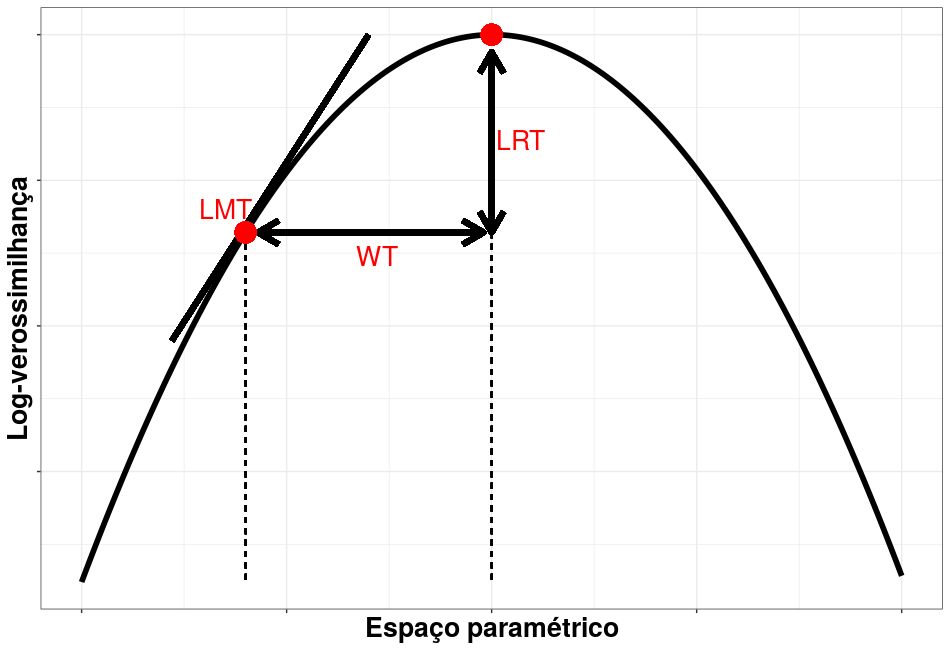
\includegraphics[width=11cm]{2-literatura/th_950_650.png}
\centering
\caption{Representação gráfica do teste da razão de verossimilhanças (LRT), teste Wald (WT) e teste escore (LMT)}
\label{fig:testes}
\end{figure}

\section{ANOVA e MANOVA}

Quando trabalhamos com modelos univariados, uma das formas de avaliar a significância de cada uma das variáveis de uma forma procedural é através da análise de variância (ANOVA) \citep{anova_fisher}. Este método consiste em efetuar testes de hipóteses sucessivos impondo restrições ao modelo original. O objetivo é testar se a ausência de determinada variável gera um modelo significativamente inferior que o modelo com determinada variável. Os resultados destes sucessivos testes são sumarizados numa tabela: o chamado quadro de análise de variância. Em geral, este quadro contêm em cada linha: a variável, o valor de uma estatística de teste referente à hipótese de nulidade de todos os parâmetros associados à esta variável, os graus de liberdade desta hipótese, e um p-valor associado à hipótese testada naquela linha do quadro.

Trata-se de um interessante procedimento para avaliar a relevância de uma variável ao problema, contudo, cuidados devem ser tomados no que diz respeito à forma como o quadro foi elaborado. Como já mencionado, cada linha do quadro refere-se a uma hipótese e estas hipóteses podem ser formuladas de formas distintas. Formas conhecidas de se elaborar o quadro são as chamadas ANOVAs do tipo I, II e III. Esta nomenclatura vem do software estatístico SAS \citep{sas}, contudo as implementações existentes em outros softwares que seguem esta nomenclatura não necessariamente correspondem ao que está implementado no SAS. No software R \citep{softwareR} as implementações dos diferentes tipos de análise de variância podem ser obtidas e usadas no pacote \emph{car} \citep{car}.

Geralmente, no contexto de modelos de regressão, para gerar o quadro de análise de variância, uma sequência de testes de testes da razão de verossimilhanças são realizados para avaliar o efeito de cada variável explicativa do modelo. Contudo é possível gerar quadros de Análise de Variância através do teste Wald. 

Do mesmo modo que é feito para um modelo univariado, podemos chegar também a uma análise de variância multivariada (MANOVA) realizando sucessivos testes de hipóteses nos quais existe o interesse em avaliar o efeito de determinada variável em todas as respostas simultaneamente. Portanto, a pergunta que a ser respondida seria: esta variável tem efeito diferente de 0 para todas as respostas? A MANOVA clássica \citep{manova} é um assunto com vasta discussão na literatura e possui diversas propostas com o objetivo de verificar a nulidade dos parâmetros de um modelo de regressão multivariado, como o $\lambda$ de Wilk's \citep{wilks}, traço de Hotelling-Lawley \citep{lawley}; \citep{hotelling}, traço de Pillai \citep{pillai} e maior raiz de Roy \citep{roy}. Tal como no caso univariado basta, para cada linha do quadro de Análise de Variância, especificar corretamente uma matriz $\boldsymbol{L}$ que represente de forma adequada a hipótese a ser testada.